\chapter{Discussion}
\label{chap:discussion}
\begin{comment}

Combine with results? why not what part.

Look into what we observed, did we get expected results based on the theory? Why? what limitations did we have for testing? Was there anything weird? What does the theory say we should expect vs. what we saw? 
Sample efficiency, convergence guarantees, changing hyperparameters, actor loss reflected in critic for ppo, the gradient magnitude and divergence, the solution space, the stages of convergence, local optima.
What does the best result say about the algorithm, our reward structure, and structure of experiment? Why did one algorithm outperform the other -- was it expected? Lucky? How did we obtain our best model and how does it reflect in the training and performance. 

Start with DDPG internal discussion, then PPO, then compare the differences between the two. Can we reach a conclusion? Under what assumptions? How critical are we to our experimental setup? 

If time, how could we improve our tests, what would be interesting to find out? 
Show some experiments that verify our thoughts, why it didn't work or why it did. Not enough time, tuning the reward, changing episode structure.

Hyperparameters are NN design parameters that generally affect the optimisation process of the network and ultimately the performance of the model. 
\end{comment}

\section{Size of the Neural Network and Replay Buffer in DDPG}
\label{sec:6_sizeof_NN}

From the training results of DDPG shown in Section \ref{sec:5_ddpg_training}, we saw that increasing the network size significantly was beneficial when compared to the Previous NTNU model, but not when compared to the Modified one. To look into why, we first need to understand this hyperparameter.

So initially, the result based on the network size was unexpected. Rather, what we expected was a something similar to for example deep learning, where we can often just increase the complexity of our model and expect better results in for example, image classification. This is because the model should be able to understand the input space better. To go a bit more into detail, the size of a NN generally correlates to its \textit{generalisation potential}. The greater the number of neurons per layer (width) or the greater the number of hidden layers (depth), there is an exponentially increasing number of parameters that can be used to parametrise the function. 
The idea is that when a NN receives increasingly complex data as input, the NN should be large enough such that it is able to ``understand'' the distribution of the input space or be able to extract higher-level information (features) through the hidden layers of the network \cite{DLUnipd}. The mechanics within NNs are relatively poorly understood however \cite{XAI}, though there is emerging research that focuses on establishing NN size design laws, such as \textit{the law of robustness} in for example \cite{bubeck2021aLawOfRobustness}.
The trade-off when increasing the size of the network, however, is that the length of training is increased as there is a need to calculate many more gradients (in backpropagation) for the increased number of parameters.  

Yet, we saw that despite having a longer training time, the performance was still not matching that of the Modified model. Furthermore, as this project was conducted, we found that our input space was quite simple in comparison to other papers, such as in \cite{song2021droneRacing} which had an input dimension of 18. Thus, our view on the size of the network greatly resonates with \cite{ControlofQuadrotorRL}, who states \textit{neural networks are quite versatile and can cope with variety of problems with a single structure.}

So, in my opinion, there is one main explanation for the difference in performance: the effect caused by the other  hyperparameter which differs among the two models, namely the \textit{size of the replay buffer R}.

Since DDPG learns off-policy by sampling experiences from its replay buffer, the agents behaviour correlates with experiences it has in its replay buffer. So, the idea is that if there are a lot of good-action experiences in the relay buffer, we expect DDPG to learn this behaviour quite quickly since it has a good probability of sampling these experiences when sampling uniformly across the buffer. If there are only a with few good-action experiences, we imagine that DDPG will struggle to learn what works well since these experiences are less likely to be sampled. Also, as training proceeds, we do expect that the agent does improve, such that the experiences stored later in the replay buffer are less random but rather good actions with more ``conviction''. So since the replay buffer is a sliding window of the agent's last experiences, we expect that a small replay buffer to only hold relatively good new experiences, while large ones contain many old ``bad'' actions. 

As a result, the size of the replay buffer thus influences the \textit{speed of learning} in DDPG, such that we expect agents with smaller replay buffers to train faster. Yet, we cannot have a too small replay buffer for two reasons: we do not wish to converge to some local optima, and we need i.i.d. samples as described in Section \ref{subsec:DDPG_Innovations}. So, there is therefore also a trade-off with stability.
Thus, the use of a larger replay buffer in the Original model could be an explanation of why it was outperformed by the Modified model -- primarily because it was learning slower. So, for further work, this can be confirmed experimentally.

\section{Learning Rate and Stability in DDPG}
\label{sec:6_learningrate_DDPG}
The learning rate for DDPG proved to have a profound effect in the learning of the DDPG models, being the only hyperparameter separating the best Modified model and the worst Previous NTNU model.

This was a good validation of the theory behind the learning rate, which is that increasing the learning rate can allow networks to converge to better performances, by essentially not getting ``stuck'' in the optimisation space. This is quite certainly the reason why the Previous NTNU model does not improve and maintained an almost constant average return, despite not having an ``optimal'' behaviour.

Yet, the extent of improvement by simply increasing the learning rate was quite unexpected since increasing the learning rate too high could lead to convergence in a local optima or instability due to large gradient updates. The reasons why this did not happen could be justified with two related reasons. The first could be because the learning rate in the Previous NTNU model was unnecessarily low, while the second could be due to stable design of DDPG through its use of target networks. This makes sense because after every large update, due to the soft update rule, the target NNs only change with a weight $\tau = 0.001$, which counteracts the initially large update. As a result, this also explains why training times are long in comparison to PPO, where the relatively fast Modified model required more than 800 epochs ($\approx$10 hours) for the critic network to converge.

\section{Size of the Trajectory and Learning Rate in PPO}
\label{sec:6_sizeof_trajectory}
Quite early in the project, the idea of increasing the length of the trajectory seemed like a good idea. An idea was that, similarly to the effect of the DDPG's replay buffer, PPO's trajectory $T$ served as a type of on-policy replay buffer. This thought was further supported by the fact that agents learning continuous robotic tasks often required more experiences to reflect the larger state and action spaces, which can be seen in the Appendices of \cite{PPO} and \cite{ppoOnDota2020}. 

The underlying theory is that increasing the batch size should improve stability. This is because the gradients calculated are averaged across a larger number of experiences, which reduces noise and variance in gradient updates \cite{batchsizeInvariance}.
By changing the batch size from 2000 to 4000 (though not seen in this project), we achieved much better performances overall which confirmed our initial theory. From Section \ref{sec:5_PPO}, we saw a further increase of the batch size from 4000 to 8000 generally provides good results, and is recommended if an increase the number of optimisation epochs and number of minibatches is desired.

In \cite{batchsizeInvariance}, it is mentioned that increasing the batch size by a factor 2 should be equivalent to reducing the Adam learning rate by a $\sqrt{2}$. This was tested by reducing the learning rate from 3e-4 to 2e-4 with a model 4-44, which produced surprisingly poor results compared to doubling the batch size in 8-44. Anyways, this was still explored with $\alpha$ lowered to 1e-5 in steps, but with similar poor training. Hence, the claim by \cite{DeepLearningBook}, and reiterated in \cite{batchsizeInvariance}, that ``the most important hyperparameter is the learning rate'', could not be verified in the same way as for DDPG, with the reason for this being uncertain. Thus, further testing in along this path was abandoned and efforts were focused on the varying the batch size, consolidated by \cite{dontdecayLRIncreaseBatch}. Nonetheless, as further work, a deeper analysis into why we did not manage to utilise the learning rate properly should be made and more testing of the PPO learning rate should be done.


\section{Speed of Learning and Anomaly Runs in PPO}
\label{sec:6_speed_of_learning_anomaly_runs}
There were a variety of hyperparameters that influenced the training speed in PPO; these were the number of optimisation epochs, number of minibatches, value coefficient and, to some extent, the entropy coefficient. 

One rather unexpected effect of increasing the speed of learning, particularly in the number of optimisation epochs and number of minibatches, was that there was an increased number of anomaly runs -- runs with dramatically poor performance as a result of the agent flying into the distance. The frequency of these inconsistent runs increased simultaneously as the non-anomaly (adjusted) performance improved.

An explanation for this follows from the on-policy learning of PPO. Since PPO learns through gaining experience from its recent and proximal (close) policy, the actions taken from a known state-space should be relatively similar. This means that when making larger updates, through an increased number of gradient updates, sort of enforces PPO to commit to its idea of a ``good'' behaviour. However, given that PPO is on-policy, this means that future experiences sampled from the environment are less exploratory in nature, which potentially makes PPO commit to a locally optimal solution as it most likely had no time to find an alternative. These larger updates can be thought of as going all-in on a locally optimal solution, while a more conservative model, such as 8-84EV, requires a longer time to reach this same point, but gathers more experience as a result.

Therefore, in the results for the PPO tests, a possible theory is that the simple waypoint navigation task is essentially a known state-space for these PPO models, such that a locally optimal solution in a fast-trained model outperforms a conservative model which does not commit to the same local optimum to the same extent. 
This can be the reason why the fastest models, such as 8-158EV, also have the highest average returns in training.
However, in the random event that the fast-trained agent ends up in some unknown state, we see that the it does not have the experience to handle this and flies off, resulting in many anomaly runs with a very negative average return. On the contrary, for the conservative model 8-84EV, we saw in \cref{table:5_PPO_test_bestModels} that it essentially had no anomaly runs, which suggests that this random anomaly event was very unlikely, which could be explained by its increased experience in training. 



\section{Underperformance and Divergence in PPO}
\label{sec:6_underperformance_divergence_PPO}

One of the biggest unmet -- and perhaps, in hindsight, naive -- expectations was that training a PPO agent should be an easy task. The reason for this was largely due the benefits of on-policy methods, which includes faster training by, ``ignoring uninteresting parts of the space'' and ``faster initial planning'' \cite{suttonAndBartoBook}, better data-efficiency \cite{PPO}, but also because of ``stronger convergence results'' when sampling on-policy \cite{suttonAndBartoBook} and the supposed, ``guaranteed monotonic improvement'' from trust-region based policy optimisation \cite{TRPO}.

\subsection{Understanding the Local Optima}
One of the reasons why this has been difficult is natural: hyperparameter tuning in deep reinforcement learning is highly sensitive \cite{selftuningAC}. This is due to the fact that reinforcement learning tasks has often a complicated state-action space, along with a few loss functions in e.g. actor-critics, that results in a very complex optimisation space. 

A prevalent example of this has been in the existence of a local optima for all PPO models. This local optima proved to be a satisfactory temporary solution for the PPO agents, but also led to an immediate divergence in training. To get an intuitive understanding of this, the path to the local optima represented where the agent had ``figured out'' that accelerating to the goal resulting in high rewards. However, as it learned to reach the goal faster and faster, it had not yet learned to brake properly, such that after reaching its peak average return, the models were continuously overshooting the goal and receiving very negative rewards. From a state-space perspective, this local optima makes sense too. Initially, all that should be learned is to point the acceleration vector $\a_t$ in the direction of the position vector $\p_t$. However, the next step for the agent is perhaps more unintuitive for the agent, which is to point $\a_t$ in the opposite direction of $\p_t$, when $\p_t$ is small and $\v_t$ is large. 

So this is an explanation for why we observed such a significant drop in the average return after each peak in the training plots. However, a natural follow-up would be to ask \textit{why did there have to be a divergence?} In other words, why did we not see a monotonic improvement during training, like in for example the Optimal model? 

\subsection{High Actor Loss at the Local Optima}
If we consider the training plots for PPO again, we noticed a strange observation in the actor loss plots: that the actor loss was increasing before each peak in average return, though at the same time, the average return was increasing and the critic loss decreasing. 
If we consider again what the actor loss represented, a large positive value signified that the advantage $\hat{A}_t$ was very negative, such that the agent was performing very poorly. So looking at Equation \eqref{3_5_advantage}, if the critic value estimate $V_{\bt}(s)$ was quite accurate, this would mean that the agent was simply choosing actions that resulted in a very poor negative $Q(s,a)$. 
So how can we explain consistently poorer agent actions, when we observe an increasing average return? 

Well, a possible justification, which was not apparent in the training plots, could be made from the existence of these \textit{anomaly runs} that we saw during testing. And as explained in \ref{sec:6_speed_of_learning_anomaly_runs}, these were increasingly common in the fastest models, despite the average return increasing. 
So we can imagine that as the agents approach their local optima, overshooting the goal became more common, and for each overshot there was a chance of it becoming an anomaly run.
Therefore, in a batch of 4000 or 8000 episodes, we can expect that the very negative rewards received from these anomaly runs were then resulting in very negative advantage estimates and spikes in the actor loss.

\subsection{Large Updates in the Optimisation Space}
Now, to go back to the question of divergence, we can try to understand the role of large updates in the optimisation space. The idea of performing gradient ascent in the actor-objective-function solution space can be thought of as hiking up a ridge between many tall mountains. 

We can then imagine that when approaching a peak (perhaps a sharp maxima), the ridge becomes thinner and its sides become steeper. In this scenario, it is intuitive that we wish to take smaller steps, as to not fall down the mountain ridge. 
However, as explained in the the previous section, what happens is the opposite: the actor loss becomes increasingly high which translates to large gradient updates -- large steps near our mountain peak. So naturally, our training process is unstable and making too big a step and falling off the ridge is inevitable given the very high actor loss near the local optima.

\subsection{Possible Improvements}
\label{subsec:6_possible_improvements}
From this discussion, it seems almost clear that attempting a much lower learning rate should be the key achieving a good PPO performance. But, as already discussed, this was attempted with no success. Also, after the Optimal PPO model was achieved with a model 4-44, it seemed like we were in the right parameter space to achieve good PPO performances and we did not need to lower the learning rate. 

Alternatively, it can be argued that training more conservative models, such as 8-84EV, rather than fast models 8-158EV, is beneficial because of the lack of anomaly runs. Though, as we observe in \cref{fig:5_training_ppo_bestModels}, even when training a model 4-44 resulted in divergence, despite having lower actor losses than 8-84EV. 

What we can conclude from this, is that the tuning the many hyperparameters of PPO is complicated and excessive tuning will not guarantee an optimal solution. Furthermore, due to the complex optimisation space and the existence of the local optima -- the lack of exploration in PPO due to the nature of its on-policy sampling presents a major problem. As we have seen, no matter how drastic hyperparameters are tuned, we always converge to the same local optima and diverge shortly after.

Therefore, there are three major improvements that can be made to this implementation. 
\begin{enumerate}
    \item Reduce the rate of learning by finding out how to reduce the learning rate properly. Too much focus was put into reaching a good solution early on, which constantly led to the convergence of a local optimum.
    \item Due to the complex optimisation space, a lucky initialisation can play a large role in finding a globally optimal solution, seen for example in the Optimal model. Thus, parallel initialisation would be a large step in the right direction.
    \item Since we have such a predominant local optima when training our PPO models, another consideration is to alter the implementation of this experiment slightly, such it is easier to find a globally optimal solution.
\end{enumerate}
As an example of altering the implementation, one could for example add 5 seconds extra to episodes and remove the termination condition when reaching the goal. This simple change should the local optima, since the models have plenty of time to reach the goal state and will not learn to accelerate excessively to the goal. 
By testing this hypothesis, the models in Table \ref{table:6_experimental} were used. Analysing their performance is out of the scope of this project, but the hypothesis was verified, where a goal rate of 99\% and RMSE of 0.0151 was achieved for model 14, and a rate of 94\% and RMSE of 0.0498 was achieved for 13.
\begin{table}[hbt]
    \centering
    \resizebox{\textwidth}{!}{%
    \begin{tabular}{||M{0.6cm}|M{2cm}||M{1.8cm}|M{1.8cm}|M{1.7cm}|M{1.4cm}|M{1.4cm}|M{1.4cm}||}    \hline
ID & Model    & Trajectory, T & Learning rate $\alpha$  & N. opt. epochs, K & N. minibatches & Ent. coef. $c_2$ & VF coef. $c_1$  \\ \hline\hline
13 & ER8-44EV & 8000          & 3,00E-04                      & 4                 & 4 & 1              & 0,01              \\ \hline
14 & ER8-88EV & 8000          & 3,00E-04                      & 8                 & 8 & 1              & 0,01              \\ \hline
    \end{tabular}
    }
    \caption{Experimental models with extra Time and no reward limit when reaching goal.}
    \label{table:6_experimental}
\end{table}

\section{Agent Behaviour with $\pm10\%$ Mass}
\label{sec:6_behaviour_robustnessTest_pm10}

In Figures \ref{fig:ddpg_test_robust}, \ref{fig:5_testing_robust+10_PPO} and \ref{fig:5_testing_robust-10_PPO} of the DDPG and PPO robustness test, we observed a clear decrease in performances when the quadrotor weight was altered. This was in contrast to our initial guess that a $\pm 10\%$ mass difference was quite a conservative robustness test. 

In my opinion, it is not exactly clear why changing mass should cause an effect in the agent performance. I would argue that since the agent is commanding accelerations to guide the quadrotor motion, what we expect it to learn is simply just a kinematic relationship -- the relationship between acceleration, velocity and position. However, this relationship, by definition, is independent of the forces acting on the quadrotor, or its kinetics. To take a simple example, the gravitational acceleration of Earth is defined as 9.81ms$^{-2}$. This acceleration is completely irrespective of mass, such that a 1kg or 10kg mass will accelerate identically at 9.81ms$^{-2}$ towards Earth in a vacuum. Following the same idea, if the quadrotor has learned to map positions and velocities to accelerations, the effect of the commanded acceleration on a quadrotor of mass 1kg or 10kg should be identical. 

Yet, this theory does not fit our observations. We see clearly that the mass does have an effect on the quadrotor behaviour, despite the agent commanding acceleration. A natural direction could be to then discuss possible reasons for why the actual accelerations are not matching the commanded ones. First, we can look at is the physical relationship between acceleration and mass. 
Essentially, the motion of the quadrotor is caused by the generalised forces acting along the $xyz$-axes, known through Newton's second law of motion $\a = \boldsymbol{f}/m$. This relationship matches the observed behaviour, where the mass acts like a \textit{gain}, such that the same commanded accelerations are mapped to smaller forces in the $+10\%$ mass case and larger forces for $-10\%$. 
For this to be true, it means that somewhere in the control loop, there exists a fixed mapping between acceleration and generalised force which does not get updated when there is a change in mass. Based on the rigid-body dynamics in Section \ref{sec:4_2_dynamics}, we know this is not true. Instead, the underlying PD-controller is designed such that the commanded accelerations are translated into desired pitch and roll angles, $\theta_d$ and $\phi_d$. Then, the PD-controller should generate the thrusts to ensure $\theta = \theta_d$ and $\phi = \phi_d$ such that we achieve the accelerations we desire. But, in equations \eqref{4_2_udot} and \eqref{4_2_vdot}, we see that there is in fact another mapping which includes the mass -- the mapping of desired accelerations to the pitch and roll angles. From these equations, we understand that if the mass of the quadrotor should change we expect that the desired pitch and roll angles should also change: a fixed acceleration should map to a larger pitch and roll angle in the $+10\%$ mass case, and the same acceleration should map to a smaller pitch and roll angle in the $-10\%$ case.
So if the mass of the quadrotor is changed directly in the simulator, but not registered in the controller, this could lead to accelerations which are not planned by the agent, which is a possible source of error.

This theory is supported by the -10\% case in Figures \ref{fig:ddpg_test_robust} and \ref{fig:5_testing_robust-10_PPO}, where we see that the quadrotor accelerates excessively in all axes, overshooting the goal position. If we consider the +10\% mass case, we see that this theory also holds to some extent. We observe in Figures \ref{fig:ddpg_test_robust} and \ref{fig:5_testing_robust+10_PPO} that generally takes a bit longer time to reach the goal position in all axes, for example taking less 3 seconds in all axes compared to about 4 seconds in average when 10\% mass was added for DDPG.
Furthermore in \cref{fig:5_testing_robust+10_PPO}, we observed that the PPO models exhibited some oscillatory behaviour along $z$, despite flying quite below the goal height. To explain this, we first have to note an interesting observation in the initialisation of the simulator.
\begin{figure}[H]
     \centering
     \begin{subfigure}[b]{0.49\textwidth}
         \centering
         \captionsetup{justification=centering}
         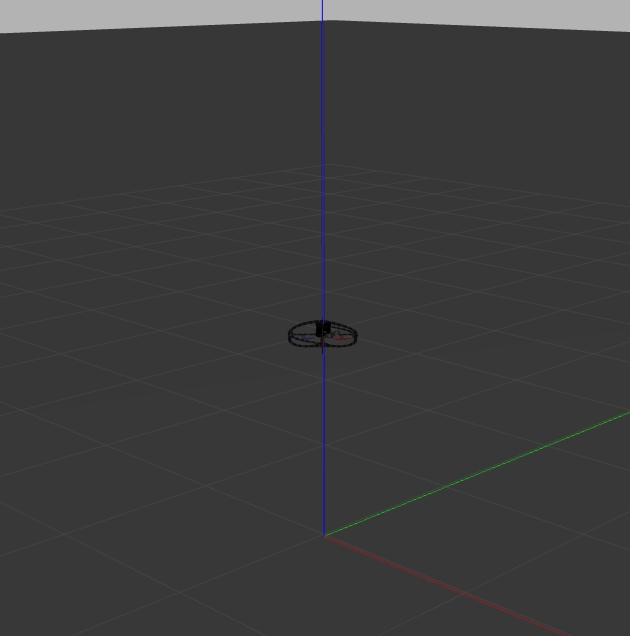
\includegraphics[width=0.72\textwidth]{figures/6_/quadrotor+10.png}
         \caption{Position of quadrotor when initialised with +10\% mass.}
         \label{fig:6_quadrotor+10}
     \end{subfigure} 
     \hfill 
    \begin{subfigure}[b]{0.49\textwidth}
         \centering
         \captionsetup{justification=centering}
         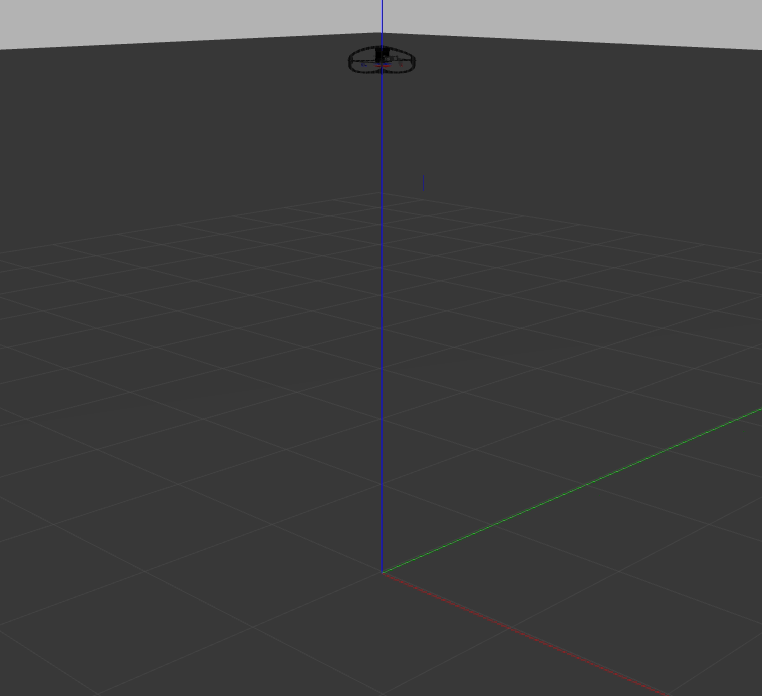
\includegraphics[width=0.8\textwidth]{figures/6_/quadrotor-10.png}
         \caption{Position of quadrotor when initialised with -10\% mass.}
         \label{fig:6_quadrotor-10}
     \end{subfigure} 
    \caption{The change in initialised position when altering the weight of the quadrotor.}
    \label{fig:6_quadrotor_mass}
\end{figure}
In \cref{fig:6_quadrotor_mass}, we observe that there is significant height difference in the initialisation position of the quadrotor. We see that when the mass is increased, there is a large negative constant deviation from the desired height, while for the -10\% mass case we see a large positive constant deviation from the desired height.
Knowing that the underlying controller for position is a PD-controller, we can therefore conclude that the is some sort of feedforward gravity term which does not get updated when the mass is changed, resulting in the constant deviations. Thus, in \cref{fig:5_testing_robust+10_PPO}, the reason the agent is not able to reach the goal is not because it is not accelerating upwards, but because the underlying PD controller is not able to regulate its height due to the unbalanced gravitational force.

To explain the oscillatory behaviour in the figure, we can guess that  it occurs because the agent thinks that it will reach the goal with some certain acceleration, and once it reads a change in velocities, it stops to not overshoot. However, since the PD controller is not compensating for the gravity term, the quadrotor instead decelerates due to gravity and starts falling down, such that the agent is constantly accelerating upwards and not reaching goal.

Another reason for why there could be a discrepancy between the actual and commanded accelerations could be in the bandwidth separation between the agent's choice of actions and the control bandwidth of the system. For a PD-controlled quadrotor, its closed-loop dynamics could be compared to a mass-spring-damper system such as \cite{Fossen2021}:
\begin{align}
    m\Ddot{x} + K_d\Dot{x} + K_p\Tilde{x} &= 0 \\
    \Ddot{x} + 2\zeta\omega_n\Dot{x} + \omega_n^2 &= 0
\end{align}
With this, the relative damping factor and natural frequency of the system is given by:
\begin{equation}
    \zeta = \frac{K_d}{2m\omega_n}, \qquad \omega_n = \sqrt{\frac{K_p}{m}}
\end{equation}
From this, we see quite clearly that the closed-loop frequency of the controller is inversely proportional to the mass. This means that when the mass is altered, the speed (time constant) of the system also changes.
As a result, when the mass of the quadrotor increases, there is a possibility that the PD-controller struggles to keep up with the agent actions, such that the agent behaviour is impaired. This agent-to-controller time-delay due to slow dynamics in the feedback loop could also help to explain why there are low frequency oscillations in \cref{fig:5_testing_robust+10_PPO}, rather than just a constant deviation.
On the contrary, when there is less mass there is a sufficient bandwidth separation so this theory does not apply. Yet, another possible consequence is that a perfectly tuned PD-controller would become underdamped if the mass decreases, which could then lead to an unstable oscillatory system if it the physical quadrotor cannot keep up, which has its own slower time constant.
